
\section{Sensor Setup}

\begin{figure}[h]
   \centering
   \begin{minipage}{0.5\textwidth}
       \centering
       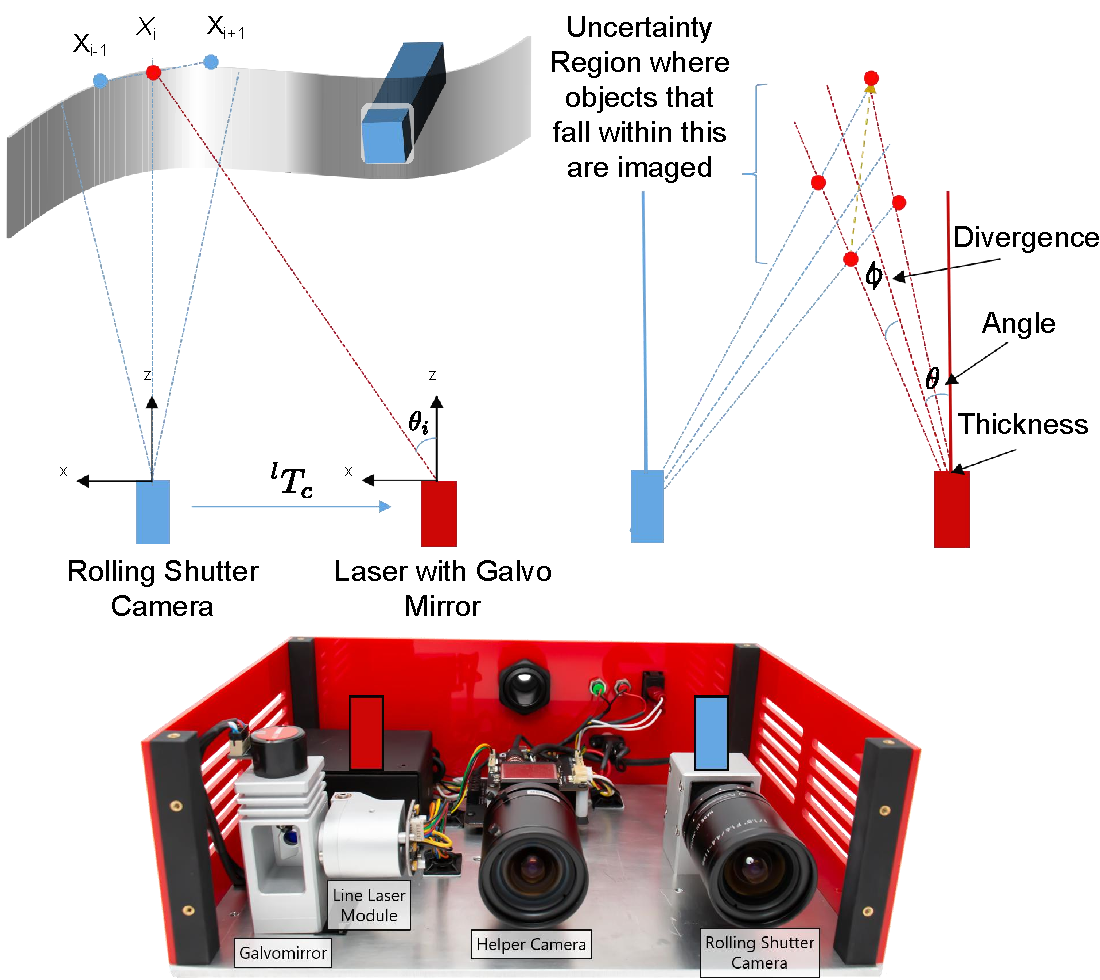
\includegraphics[width=1.0\textwidth]{figures/LC.pdf} % first figure itself
   \end{minipage}\hfill
   % \begin{minipage}{0.3\textwidth}
   %     \centering
   %     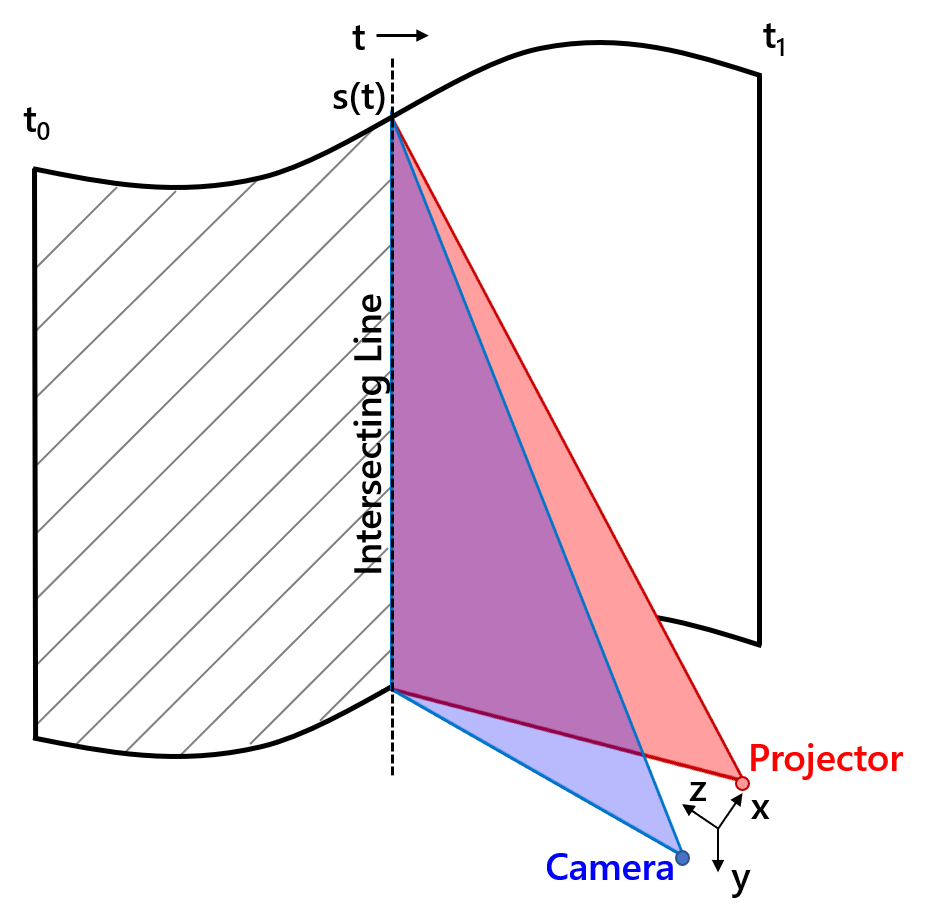
\includegraphics[width=0.9\textwidth]{light_curtain_iso.png} % second figure itself
   % \end{minipage}
   \centering
   \caption{ \textbf{Below:}  Our Adaptive Sensor of choice, the Triangulation Light Curtain Device (LC) \cite{bartels2019Agile}, consisting of a laser, galvomirror and NIR camera. \textbf{Above:} The light curtain senses a ruled 3D surface extruding from a given top-down 2D curve we call a curtain. Surfaces that fall within the \textit{thickness} of the curtain, result in higher intensity shown in the NIR image.}
   \label{fig:lcdevice}  
\end{figure}

\begin{figure}[h]
    \centering
    \begin{minipage}{0.5\textwidth}
        \centering
        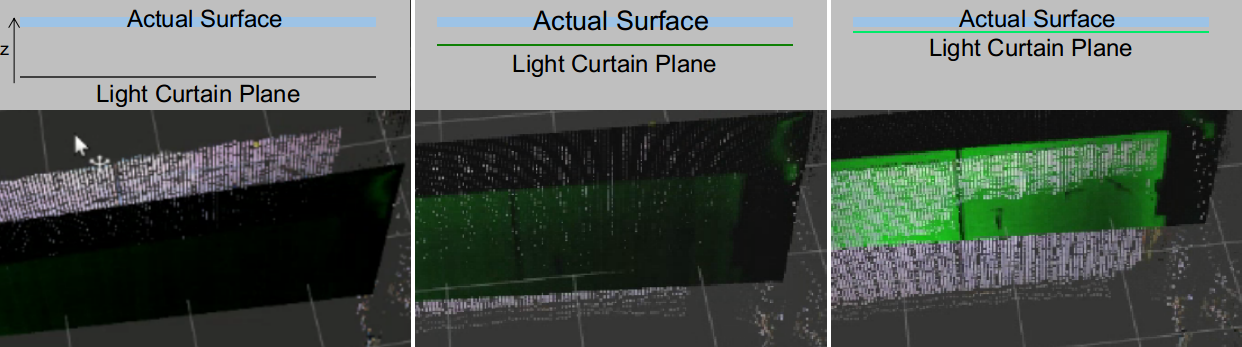
\includegraphics[width=1.0\textwidth]{figures/planesweep.png} % first figure itself
    \end{minipage}\hfill
    % \begin{minipage}{0.3\textwidth}
    %     \centering
    %     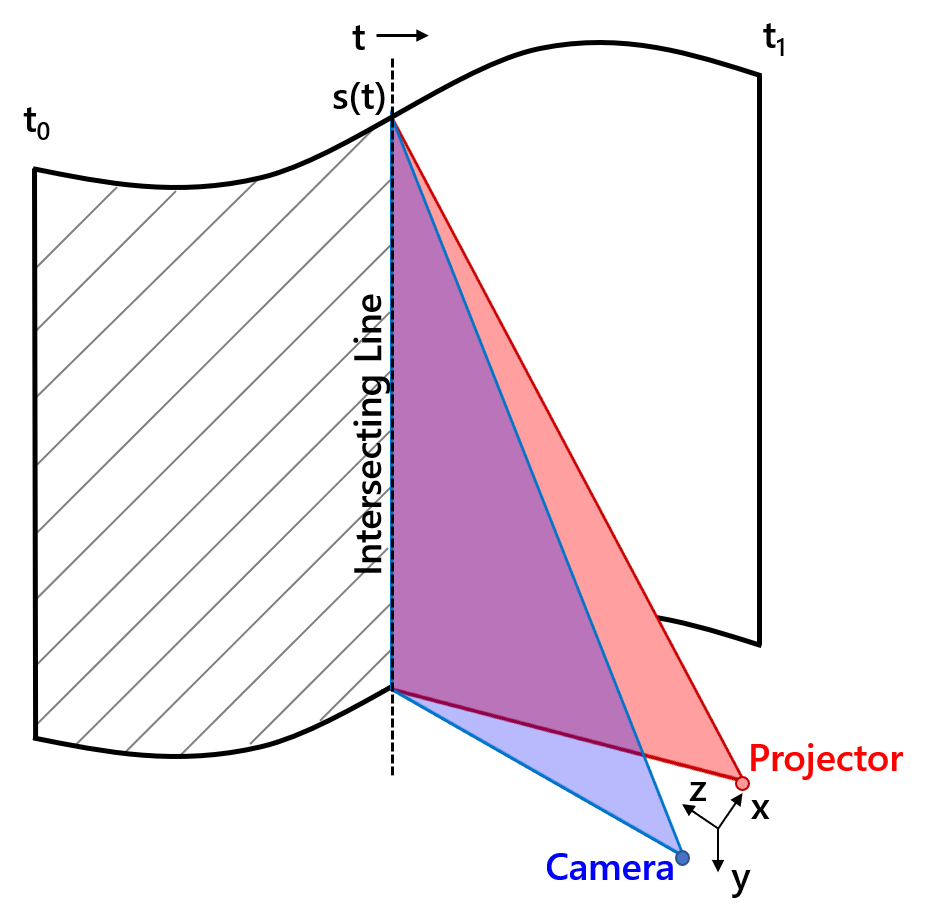
\includegraphics[width=0.9\textwidth]{light_curtain_iso.png} % second figure itself
    % \end{minipage}
    \centering
    \caption{Here, we sweep a planar 3D ruled surface or curtain across at various depths. As the curtain surface approaches the true surface, the intensity value slowly increases on the NIR image, due to the sensing location and curtain thickness. One can see how we could adaptively sense a scene to converge on the real depth with our device.}
    \label{fig:planesweep} 
 \end{figure}

The Light Curtain device consists of a rolling shutter NIR (Near-Infrared) camera rotated 90$\degree$ (that images planes in the world per pixel column), a Line Laser module and a Galvomirror (that generates planes of light in the world depending on the angle). The exact sensing location is obtained by intersecting (triangulating) these two planes, and sweeping this laser line creates a 3D ruled surface called a curtain. We can place a curtain along any surface by controlling the galvo and rolling shutter speed subject to it's constraints, making it adaptive in nature. Do note that the image and laser planes have some divergence, so their intersection results in a volume in space (bounded by purple points in Fig~\ref{fig:lcdevice}) with some \textit{thickness}, where any objects that intersect it result in higher intensities in the NIR image. This means that as the sensing location approaches the true surface, pixel intensities on NIR image increases (Fig.~\ref{fig:planesweep}). 

\begin{figure}[h]
   \centering
   \begin{minipage}{0.4\textwidth}
       \centering
       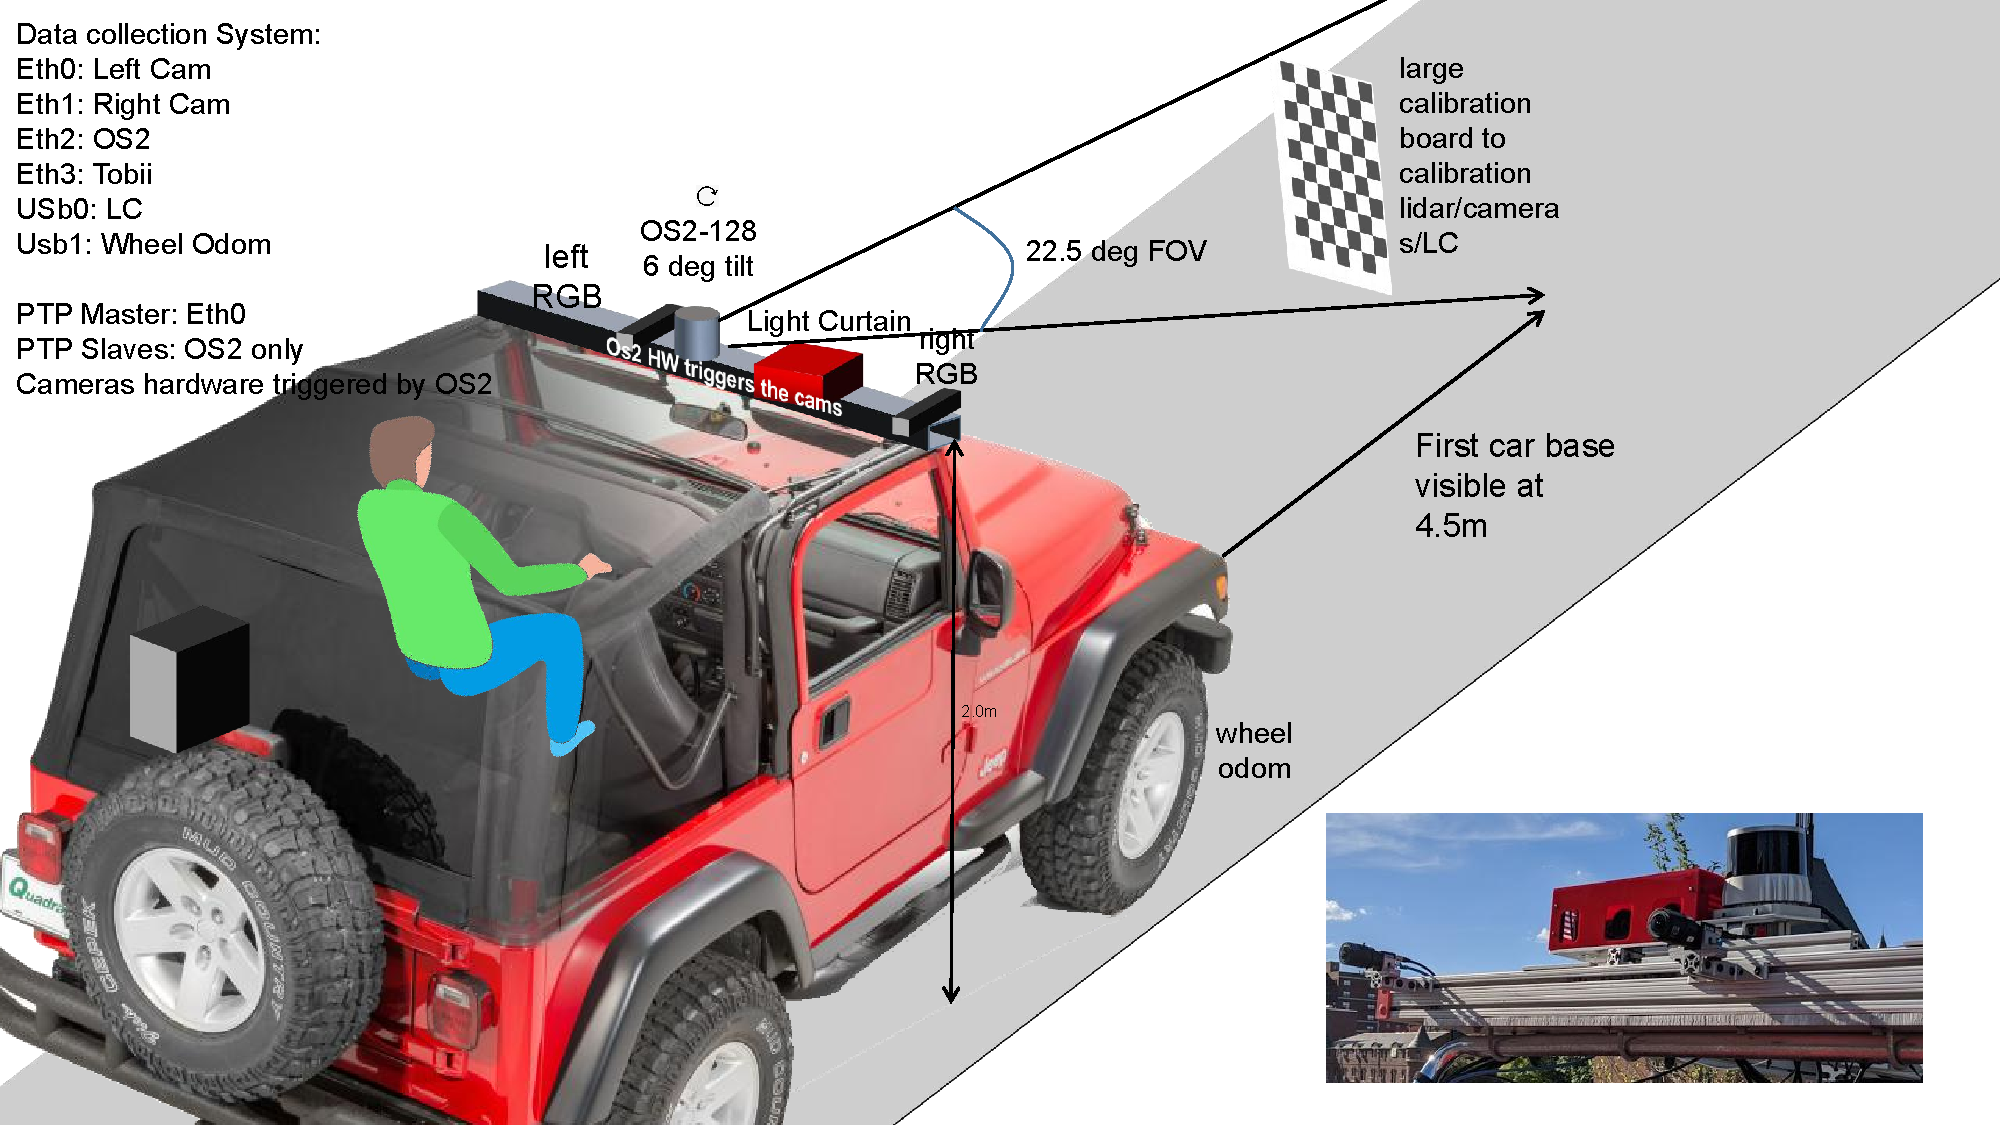
\includegraphics[width=1.0\textwidth]{figures/array.pdf}
   \end{minipage}\hfill
   \centering
   \caption{Setup for real-world experiments: FLIR Stereo camera pair, Light Curtain (LC) and OS2-128 Lidar used for ground truth validation.}
   \label{fig:sensorarray} 
\end{figure}

Real-world experiments are conducted using our array of sensors consisting of an RGB Stereo Camera Pair, Light Curtain device, and a 128 Beam Lidar for accuracy validation and later RGB depth estimation network training (Fig.~\ref{fig:sensorarray}). Simulated experiments are also conducted with KITTI dataset \cite{Geiger2013IJRR}, through a Light Curtain Simulator that uses the ground truth depthmap along with control in NIR instrinsics, Laser extrinsincs, Galvomirror speed, Laser Divergence/Thickness and Angle. 

% \begin{figure}[h]
%    \centering
%    \begin{minipage}{0.5\textwidth}
%        \centering
%        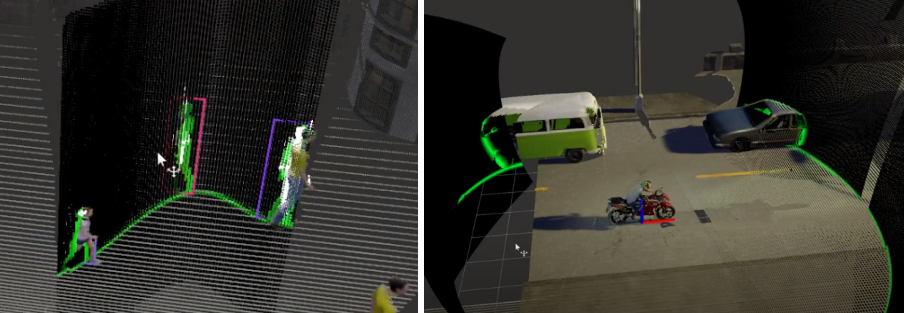
\includegraphics[width=1.0\textwidth]{figures/sim.png}
%    \end{minipage}\hfill
%    \centering
%    \caption{Light Curtain Simulator}
%    \label{fig:lcsimkitti} 
% \end{figure}
%\vspace{-.1in}


